\documentclass[10pt,openright,twoside,french]{book}

\input philippe2013
\input philippe2013_cours
\input philippe2013_sections
\input philippe2013_chapitre
\renewcommand\PartProgramme{Géométrie}
\renewcommand\MaCouleur{Purple}

\pieddepage{}{%
\begin{tikzpicture}[scale=0.65]
\shadedraw [top color=white, bottom color=\MaCouleur, draw=\MaCouleur]
[l-system={Sierpinski triangle, step=1pt, angle=60, axiom=F, order=6.5}]
lindenmayer system -- cycle;
\draw (30:0.65cm) node {\bfseries\textcolor{black}{\thepage}};
\end{tikzpicture}%
}{}


\setcounter{chapter}{8}
\begin{document}
\chapter[Fonctions circulaires]{Fonctions\\ circulaires}\label{fonctions_circulaires}


\section{Définitions}

On se place dans un repère \Oij. Sur le cercle trigonométrique $\calig U$, on rappelle qu'un point $M$ est repéré à l'aide de l'angle $\left(\vect\imath\pv\vect{OM}\right) = \alpha$.\par
L'abscisse du point $M$ est alors $\cos(\alpha)$ et son ordonnée est $\sin(\alpha)$.

\begin{center}
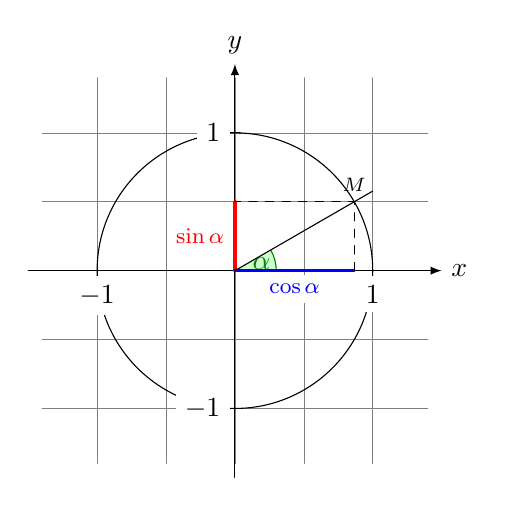
\begin{tikzpicture}[scale=1.75,cap=round]
    % Local definitions
    \def\costhirty{0.8660256}
    % Colors
    \colorlet{anglecolor}{green!50!black}
    \colorlet{sincolor}{red}
    \colorlet{tancolor}{orange!80!black}
    \colorlet{coscolor}{blue}
    % Styles
    \tikzstyle{axes}=[>=latex]
    \tikzstyle{important line}=[very thick]
    \tikzstyle{information text}=[rounded corners,fill=red!10,inner sep=1ex]
    % The graphic
    \draw[style=help lines,step=0.5cm] (-1.4,-1.4) grid (1.4,1.4);
    \draw (0,0) circle (1cm);
    \begin{scope}[style=axes]
        \draw[->] (-1.5,0) -- (1.5,0) node[right] {$x$} coordinate(x axis);
        \draw[->] (0,-1.5) -- (0,1.5) node[above] {$y$} coordinate(y axis);
        \foreach \x in {-1,1} \draw[xshift=\x cm] (0pt,1pt) -- (0pt,-1pt) node[below,fill=white] {$\x$};
        \foreach \y in {-1,1} \draw[yshift=\y cm] (1pt,0pt) -- (-1pt,0pt) node[left,fill=white] {$\y$};
    \end{scope}
    \filldraw[fill=green!20,draw=anglecolor] (0,0) -- (3mm,0pt) arc(0:30:3mm);
    \draw (15:2mm) node[anglecolor] {$\alpha$};
    \draw[style=important line,sincolor] (0,0) -- node[left,fill=white] {\footnotesize$\sin \alpha$} (0,0.5);
    \draw[style=important line,coscolor] (30:1cm |- x axis) -- node[below=1pt,fill=white] {\footnotesize$\cos \alpha$} (0,0);
    \draw[dashed] (30:1cm |- x axis) -- (30:1cm) -- (30:1cm -| y axis);
    \draw (intersection of 0,0--30:1cm and 1,0--1,1) coordinate (t);
    \draw (0,0) -- (t);
    \draw (30:1cm) node[above] {\scriptsize$M$};
\end{tikzpicture}
\end{center}

\begin{Defi}
    On définit alors les \iptb{fonctions circulaires}\index{fonction!circulaire}\index{cosinus}\index{sinus} :\par\medskip
        \textbf{Cosinus :} $\left\{\begin{array}{rcl}
                                                \R & \to & \intervalleff{-1}{1} \\
                                                x & \mapsto & \cos(x)
                                            \end{array}\right.$ \qquad et \qquad
        \textbf{Sinus :} $\left\{\begin{array}{rcl}
                                                \R & \to & \intervalleff{-1}{1} \\
                                                x & \mapsto & \sin(x)
                                            \end{array}\right.$
\end{Defi}

\begin{Exemple}
    En physique, on utilise les fonctions suivantes :
    \[\cos\left(\omega t + \varphi\right) \qetq \sin\left(\omega t + \varphi\right)\] où $\omega \in \R$ et $\varphi \in \R$.
    Le nombre $\omega$ est appelé la pulsation et $\varphi$ la phase.
\end{Exemple}

\section{\'Etude des fonctions circulaires}
\subsection{Parité}

\begin{Defi}
    Soit $f$ une fonction définie sur un ensemble $\calig D_f$.\par
    \begin{itemize}
        \item $f$ est dite \iptb{paire}\index{fonction!paire} lorsque, pour tout $x \in \calig D_f, f(-x) = f(x)$.
        \item $f$ est dite \iptb{impaire}\index{fonction!impaire} lorsque, pour tout $x \in \calig D_f, f(-x) = -f(x)$.
    \end{itemize}
\end{Defi}

\begin{Exemple}[s]
    \begin{enumerate}
        \item $f \colon x \mapsto x^2$. Alors $f(-x) = (-x)^2 = (-x) \times (-x) = x^2 = f(x)$ donc $f$ est paire.
        \item $g \colon x \mapsto x^3$. Alors $g(-x) = (-x)^3 = (-x) \times (-x) \times (-x) = -x^3 = -g(x)$ donc $g$ est impaire.
    \end{enumerate}
\end{Exemple}

\begin{Prop}
    La fonction cosinus est paire : $\cos(-x) = \cos(x)$.\par
    La fonction sinus est paire : $\sin(-x) = -\sin(x)$.
\end{Prop}

\begin{Prop}
    La courbe représentative d'une fonction paire est symétrique par rapport à l'axe des ordonnées.\par
    La courbe représentative d'une fonction impaire est symétrique par rapport à l'origine du repère.
\end{Prop}

\subsection{Périodicité}

\begin{Defi}
    Soit $f$ une fonction définie sur $\calig D_f$.\par
    $f$ est dite \iptb{périodique}\index{fonction!périodique} sur $\calig D_f$ lorsqu'il existe un réel $T$ le plus petit possible tel que :
    \[\text{pour tout } x \in \calig D_f,\quad f(x + T) = f(x).\]
    On dit que la fonction $f$ est $T-$périodique et le nombre $T$ s'appelle la \ipt{période}.
\end{Defi}

\begin{Prop}
    Les fonctions sinus et cosinus sont $2\pi-$périodiques. En effet,
    \[\cos(x + 2\pi) = \cos(x) \qetq \sin(x + 2\pi) = \sin(x).\]
\end{Prop}

\begin{Exemple}[s]
    \begin{enumerate}
        \item Montrer que $x \mapsto \tan(x) = \dfrac{\sin(x)}{\cos(x)}$ est $\pi-$périodique.
        \item Montrer que la période de la fonction $f \colon x \mapsto \cos(\omega x + \varphi)$ est périodique de période $T = \dfrac{2\pi}{\omega}$.
    \end{enumerate}
\end{Exemple}

\subsection{Signe}

Les fonctions cosinus et sinus étant $2\pi-$ périodiques, il suffit de les étudier sur un intervalle de longueur $2\pi$. Par exemple, l'intervalle $\intervalleff{0}{2\pi}$.

\subsection{Variation}

On utilise cette fois les symétries des courbes représentatives des fonctions circulaires. On les étudie sur $\intervalleff{-\pi}{\pi}$.

\end{document}
